\documentclass[12pt,a4paper,oneside]{report}

\usepackage[a4paper,margin=1in,headheight=15pt,headsep=10pt]{geometry}
\usepackage{amsmath}
\usepackage{newtxtext,newtxmath}
\usepackage{setspace}
\usepackage{graphicx}
\graphicspath{{figures/}{./}}
\usepackage{array}
\usepackage{longtable}
\usepackage{tabularx}
\usepackage{enumitem}
\usepackage{fancyhdr}
\usepackage{xcolor}
\usepackage{hyperref}
\usepackage{listings}
\usepackage{caption}
\usepackage{float}
\usepackage{titlesec}
\usepackage{etoolbox}
\usepackage{tikz}
\usetikzlibrary{arrows.meta,positioning,shapes.geometric}

\setstretch{1.3}
\raggedbottom
\setcounter{secnumdepth}{3}
\setcounter{tocdepth}{3}
\titleformat{\chapter}[block]
  {\normalfont\LARGE\bfseries\upshape\centering}
  {}
  {0pt}
  {\MakeUppercase}
\titleformat{\section}
  {\normalfont\Large\bfseries\upshape}
  {\thesection}{0.8em}{}
\titleformat{\subsection}
  {\normalfont\large\bfseries\upshape}
  {\thesubsection}{0.8em}{}
\titlespacing*{\chapter}{0pt}{-6pt}{8pt}
\titlespacing*{\section}{0pt}{1.0ex plus 0.15ex minus 0.1ex}{0.35ex}
\titlespacing*{\subsection}{0pt}{0.75ex plus 0.1ex minus 0.1ex}{0.25ex}
\titlespacing*{\subsubsection}{0pt}{0.6ex plus 0.1ex minus 0.1ex}{0.2ex}
\setlength{\floatsep}{4pt plus 1pt minus 1pt}
\setlength{\textfloatsep}{5pt plus 1pt minus 1pt}
\setlength{\intextsep}{4pt plus 1pt minus 1pt}
\setlength{\abovecaptionskip}{2pt}
\setlength{\belowcaptionskip}{1pt}
\setlength{\abovedisplayskip}{6pt plus 1pt minus 1pt}
\setlength{\belowdisplayskip}{6pt plus 1pt minus 1pt}
\setlength{\abovedisplayshortskip}{4pt plus 1pt minus 1pt}
\setlength{\belowdisplayshortskip}{4pt plus 1pt minus 1pt}
\setlength{\tabcolsep}{3pt}
\renewcommand{\arraystretch}{1.0}
\setlength{\LTpre}{3pt}
\setlength{\LTpost}{3pt}
\AtBeginEnvironment{table}{\singlespacing}
\AtBeginEnvironment{longtable}{\singlespacing}
\captionsetup[table]{skip=4pt}
\captionsetup[figure]{skip=3pt}
\hypersetup{
  colorlinks=true,
  linkcolor=black,
  urlcolor=blue,
  citecolor=black,
  pdftitle={AI Forensic Insider Risk Review System},
  pdfsubject={Mini project report}
}
\pagestyle{fancy}
\fancyhf{}
\fancyhead[R]{AI Forensic Insider Risk Review}
\renewcommand{\headrulewidth}{0.4pt}
\fancyfoot[L]{Department of Computer Applications}
\fancyfoot[R]{\thepage}
\renewcommand{\footrulewidth}{0.4pt}
\fancypagestyle{plain}{\fancyhf{}}
\lstset{
  basicstyle=\ttfamily\scriptsize,
  breaklines=true,
  frame=single,
  columns=fullflexible,
  keepspaces=true,
  aboveskip=2pt,
  belowskip=2pt
}
\setlist[itemize,enumerate]{
  topsep=0.5pt,
  itemsep=0pt,
  parsep=0pt,
  partopsep=0pt
}
\setlist[description]{
  topsep=1pt,
  itemsep=0pt,
  parsep=0pt,
  partopsep=0pt
}

\newcommand{\projecttitle}{AI Forensic Insider Risk Review System}
\newcommand{\studentname}{HRISHIKESH P S}
\newcommand{\registernumber}{MCA25MCA-2029}
\newcommand{\department}{Department of Computer Applications}
\newcommand{\collegename}{Mar Athanasius College of Engineering}
\newcommand{\collegeplace}{Kothamangalam}
\newcommand{\collegestatus}{Government Aided Autonomous Institution}
\newcommand{\guide}{Dr. Manu John}
\newcommand{\hod}{Dr. Sonia Abraham}
\newcommand{\degree}{Master of Computer Applications}
\newcommand{\academicyear}{2025--2027}

\begin{document}

\pagestyle{empty}
\pagenumbering{roman}
\begin{titlepage}
\centering
\vspace*{0.8cm}
{\Large\bfseries \MakeUppercase{\collegename}\par}
\vspace{0.15cm}
{\large \MakeUppercase{\collegeplace}\par}
\vspace{0.15cm}
{\normalsize (\collegestatus)\par}
\vspace{0.4cm}
{\large\bfseries \department\par}
\vspace{1.4cm}
{\large\bfseries MINI PROJECT REPORT\par}
\vspace{0.45cm}
ON\\[0.45cm]
{\Large\bfseries \MakeUppercase{\projecttitle}\par}
\vspace{1.2cm}
Submitted in partial fulfilment of the requirements for the award of the
degree of\\[0.3cm]
{\large\bfseries \degree\par}
\vspace{1.0cm}
Done by\\[0.25cm]
{\large\bfseries \studentname\par}
Reg. No.: \registernumber
\vspace{0.9cm}

Under the guidance of\\[0.25cm]
{\large\bfseries \guide\par}
\vfill
{\large \academicyear\par}
\end{titlepage}

\chapter*{Certificate from College}
\addcontentsline{toc}{chapter}{Certificate from College}
\begin{center}
{\Large\bfseries \MakeUppercase{\collegename}\par}
{\large \MakeUppercase{\collegeplace}\par}
(\collegestatus)\\[1.0cm]
{\Large\bfseries CERTIFICATE\par}
\vspace{0.5cm}
{\large\bfseries \MakeUppercase{\projecttitle}\par}
\end{center}
\vspace{0.6cm}
Certified that this is the bonafide record of mini project work carried
out by \textbf{\studentname}, Reg. No. \textbf{\registernumber}, during
the academic year \academicyear, in partial fulfilment of the
requirements for the award of the degree of \degree\ under APJ Abdul
Kalam Technological University.

\vspace{2.0cm}
\noindent
\begin{tabularx}{\textwidth}{X X}
  \rule{5cm}{0.4pt} & \rule{5cm}{0.4pt}\\
  \guide & \hod\\
  Faculty Guide & Head of the Department\\[1.8cm]
  \rule{5cm}{0.4pt} & \rule{5cm}{0.4pt}\\
  Internal Examiner & External Examiner
\end{tabularx}

\chapter*{Declaration}
\addcontentsline{toc}{chapter}{Declaration}
I hereby declare that this mini project report entitled
\textit{\projecttitle} is a record of the project work carried out by me.
The project implementation, analysis, and results described in this
report are presented to the best of my knowledge and are based on the
project repository and its saved evaluation outputs. This work has not
formed the basis for the award of any other degree, diploma, or similar
title. Any use of third-party datasets, libraries, or published material
is acknowledged in the report.

\vspace{1.2cm}
\noindent Place: Kothamangalam\\
Date: \hfill Signature of the Student

\chapter*{Acknowledgement}
\addcontentsline{toc}{chapter}{Acknowledgement}
I express my sincere gratitude to my mini project guide,
\textbf{\guide}, for guidance and valuable suggestions during the
development and documentation of this project. I thank
\textbf{\hod}, Head of the Department of Computer Applications, and the
faculty and staff of \collegename, Kothamangalam, for their support.

I also acknowledge the creators of the CERT Insider Threat Test Dataset
and the developers and maintainers of the open-source Python,
scikit-learn, pandas, NumPy, FastAPI, React, Vite, and Streamlit tools
used in this demonstration. Finally, I express my gratitude to my family
and friends for their encouragement.

\begin{flushright}
- \studentname
\end{flushright}

\chapter*{Abstract}
\addcontentsline{toc}{chapter}{Abstract}
This project presents a prototype for reviewing employee activity
records for patterns associated with known insider-threat scenarios.
It processes the CERT r4.2 synthetic activity logs for logons, removable
devices, file access, email, and web activity. Event records are cleaned
and aggregated to employee-day counts. The resulting numerical features
are labelled by matching employee IDs and calendar days to the r4.2
incident windows supplied in the CERT answer file. Four models are
compared: Logistic Regression, Decision Tree, Random Forest, and
Isolation Forest. A grouped train/validation/test design keeps each
employee in only one split. Models are compared using Average Precision
and precision and recall at fixed review capacities. Random Forest is
selected by validation Average Precision; a one-percent review capacity
is selected using validation F1 from a predeclared candidate grid. On
held-out test records this gives Random Forest an F1 of 0.130 (precision
9.37\%, recall 21.45\%). The five-percent operating point remains as a
reference and gives higher recall but lower precision. This is a useful
signal for a research demonstration, but not evidence of wrongdoing:
unlabelled records are not confirmed benign, incident labels are
incomplete, and the tested threshold produces many records requiring
human review. A local React dashboard, backed by a FastAPI service,
scores selected activity CSV files and presents ranked review leads.
The report explains
the data pipeline, modelling, software design, evaluation, constraints,
and responsible-use safeguards.

\clearpage
\addcontentsline{toc}{chapter}{List of Tables}
\listoftables

\clearpage
\addcontentsline{toc}{chapter}{List of Figures}
\listoffigures

\addcontentsline{toc}{chapter}{Contents}
\tableofcontents
\clearpage
\pagenumbering{arabic}
\pagestyle{fancy}
\fancypagestyle{plain}{
  \fancyhf{}
  \fancyhead[R]{AI Forensic Insider Risk Review}
  \renewcommand{\headrulewidth}{0.4pt}
  \fancyfoot[L]{Department of Computer Applications}
  \fancyfoot[R]{\thepage}
  \renewcommand{\footrulewidth}{0.4pt}
}

\chapter{Introduction}
\section{Background}
Organisations record routine digital activity in access, device,
communication, file, and web logs. Those records can help an investigator
understand when an account or device behaved unusually. The volume and
variety of logs make manual review difficult, so a data-processing and
ranking tool can help prioritise records for inspection.

This project is an educational demonstration of that idea. It converts
the CERT r4.2 synthetic activity data into daily aggregates, compares
several machine-learning approaches against known incident windows, and
provides a local dashboard to explore high-priority employee-days. A
model score is a prioritisation signal only. It does not establish intent,
identity, policy violation, or guilt.

\section{Problem statement}
The prototype needs to turn a large collection of heterogeneous activity
CSV files into a compact and inspectable review queue. The analysis must
handle missing or malformed records, combine sources at a consistent
employee-day granularity, evaluate models under severe class imbalance,
and show investigators what activity contributed to a rank. Since only
known incidents are labelled, a record outside a listed incident window
must not be described as definitively normal.

\section{Objectives of the Project}
\textbf{Aim:} Build and evaluate a local, explainable-at-the-signal-level
prototype that ranks employee activity records for human review.

\textbf{Objectives}
\begin{enumerate}
  \item Inspect and clean five CERT r4.2 activity CSV sources.
  \item Aggregate activity into daily features for each user.
  \item Create a binary known-incident-window label from the answer file.
  \item Compare three supervised classifiers and one unsupervised anomaly
        detector using employee-grouped data splits.
  \item Evaluate ranking quality at fixed review capacities, selecting
        the reported one-percent operating point using validation F1 and
        retaining five percent as a comparison.
  \item Save model artifacts and expose a local React dashboard with a
        FastAPI service for human review of new activity records.
\end{enumerate}

\section{Scope of the Project}
The implemented feature set contains daily event counts, after-hours
counts, device connection counts, and email attachment totals when those
fields exist. It does not analyse message bodies, web URLs, or file
contents. The model target is whether an employee-day overlaps a listed
incident window in the r4.2 answer file. The prototype is not a live
monitoring system, identity-resolution system, case-management platform,
or automated disciplinary tool. The primary demonstration interface is
a local React dashboard backed by FastAPI. The earlier Streamlit
interface remains available as an alternative.

\section{Project Domain and Technology Stack}
The project falls within applied data analysis, supervised classification,
and anomaly detection. Python is used for feature preparation and model
development. pandas and NumPy support tabular processing; scikit-learn
provides the estimators, grouped splitting, and evaluation metrics; joblib
stores the fitted models; React and FastAPI provide the local interactive
demonstration \cite{reactdocs,fastapidocs}; and Streamlit remains
available as an alternative. Jupyter Notebook is used for the
reproducible analysis.

\section{Organisation of the Report}
Chapter 2 reviews supporting literature and project proposals.
Chapter 3 presents system analysis, including the dataset, preprocessing,
algorithms, feasibility, and environment. Chapter 4 describes model
building and system design. Chapter 5 reports evaluation results and
discussion; Chapter 6 documents the local deployment. Chapter 7 records
selected Git history and project challenges, followed by learning
outcomes, conclusion, future work, references, and appendices.

\chapter{Supporting Literature}
\section{Literature Review}
Insider-threat detection is difficult because legitimate and harmful
activity can share the same systems and workflows. A single event such
as a late login, removable-media connection, or large email attachment
is not sufficient evidence of malicious intent. This motivates combining
contextual signals and keeping a human investigator in the decision
loop. The CERT Insider Threat Test Dataset provides synthetic user
activity and scenario labels for reproducible experimentation; its
scenarios are useful for evaluating methods but cannot represent every
real organisation or establish real-world operational accuracy
\cite{cert}.

Logistic Regression is a relatively interpretable supervised baseline.
It estimates a linear decision function over the input features and can
provide a useful comparison when the relationship between engineered
features and the label is approximately additive. A Decision Tree
represents a series of feature splits and can model simple nonlinear
relationships. Random Forest averages a collection of randomized trees,
reducing the instability of a single tree and providing a flexible
tabular-data baseline \cite{breiman}.

Isolation Forest is an unsupervised anomaly-detection method. It isolates
observations through random feature and split selection; unusual points
tend to be isolated with shorter paths \cite{liu}. In this project it is
trained without using incident labels. It answers a different question
from the supervised classifiers: ``which records are unusual in this
feature space?'' Unusual does not necessarily mean incident-related.

Evaluation must reflect both the rarity of the positive class and the
intended review workflow. Accuracy can be dominated by the majority
class. Precision measures how many alerts match known positive labels;
recall measures how many known positives were retrieved. Average
Precision summarizes precision over ranked thresholds and is useful for
rare-positive ranking tasks. The scikit-learn documentation describes
these metrics and their averaging conventions \cite{sklearnmetrics}.
This project reports results at a validation-selected one-percent
employee-day capacity and retains the five-percent queue as a larger
fixed-size comparison.

\section{Literature Review Summary}
The selected methods provide complementary baselines rather than a claim
that one algorithm is universally best. Supervised algorithms can learn
patterns represented in the known incident labels; an anomaly detector
can rank deviations without those labels. For either approach, the
quality of the labels, the feature design, the data split, and the
review capacity constrain conclusions more strongly than the algorithm
name alone.

\section{Findings and Proposals}
\begin{itemize}
  \item Evaluate per-class precision and recall rather than relying on
        accuracy alone.
  \item Keep employees disjoint across model-development and test
        partitions to reduce person-specific leakage.
  \item Select a model using validation data; reserve test data for final
        reporting.
  \item Describe non-matching labels as ``not listed in known incidents''
        rather than as a verified normal class.
  \item Require independent corroboration and accountable human review
        before acting on a flag.
\end{itemize}

\chapter{System Analysis}
\section{Analysis of the dataset}
\subsection{About the dataset}
The experiment reads the CERT r4.2 release from the local \texttt{r4.2}
folder and the matching \texttt{answers/insiders.csv} answer file. The
activity inputs are listed in Table~\ref{tab:sources}. The answer file is
used only for research labels and model evaluation/training; the
dashboard's user-selected activity folder does not need the answer file.

\begin{table}[H]
\centering
\caption{Activity source inventory}
\label{tab:sources}
\begin{tabularx}{\textwidth}{|p{0.30\textwidth}|X|}
\hline
Source & Fields used by the first-stage pipeline\\
\hline
\texttt{logon.csv} & Timestamp, user, activity records\\
\hline
\texttt{device.csv} & Timestamp, user, activity; connection events counted\\
\hline
\texttt{file.csv} & Timestamp, user, file activity records\\
\hline
\texttt{email.csv} & Timestamp, user, attachment count\\
\hline
\texttt{http.csv} & Timestamp, user, web activity records\\
\hline
\texttt{answers/insiders.csv} & Dataset version, user, incident start/end, scenario\\
\hline
\end{tabularx}
\end{table}

The saved labelled table contains 330,452 employee-days for 1,000
synthetic user IDs, covering 2 January 2010 through 17 May 2011. It
contains 1,364 positive employee-days (0.413\%) under the notebook's
labeling rule. The saved test partition has 66,118 employee-days and 289
positive labels. These are reproducible facts from the project's saved
artifacts, not general statistics about real organisations.

\subsection{Explore the dataset}
The five files contain approximately 32.77 million raw event rows. The
cleaning summary reports 32,409,354 rows kept and 360,868 duplicates
removed. No missing user IDs or invalid dates were reported in the saved
quality summary. Deduplication is performed within each input chunk, so
duplicates spanning separate chunks may remain; this is a limitation to
verify if exact global deduplication is required.

\begin{table}[H]
\centering
\caption{Data-cleaning summary from saved quality output}
\label{tab:clean}
\begin{tabularx}{\textwidth}{|l|*{3}{>{\raggedleft\arraybackslash}X|}}
\hline
Source & Rows read & Rows kept & Duplicates removed\\
\hline
Logon & 854,859 & 854,859 & 0\\
\hline
Device & 405,380 & 405,374 & 6\\
\hline
File & 445,581 & 445,581 & 0\\
\hline
Email & 2,629,979 & 2,618,056 & 11,923\\
\hline
HTTP & 28,434,423 & 28,085,484 & 348,939\\
\hline
Total & 32,770,222 & 32,409,354 & 360,868\\
\hline
\end{tabularx}
\end{table}

The positive class is highly sparse. The 1,364 positive days belong to
70 user IDs, and many users have no known positive days. A group-aware
split therefore matters: random row splitting could place records from
the same person in training and testing and produce an overly optimistic
estimate for generalization to unseen employees.

\section{Data preprocessing}
\subsection{Data cleaning}
Each CSV is read in chunks of 25,000 rows to limit memory use. Column
names and user IDs are normalized, timestamps are parsed, rows missing a
usable user or date are excluded, and duplicate rows within a chunk are
removed. Each retained record contributes to a calendar-day aggregate.
Where source fields are available, device ``connect'' events and email
attachment totals are separately accumulated. Missing source/day
combinations are filled with zero after source tables are combined.

\subsection{Analysis of feature variables}
The modelling table contains the numeric activity features below. The
model excludes user ID, date, scenario, and the target label.

\begin{table}[H]
\centering
\caption{Employee-day feature definitions}
\label{tab:features}
\begin{tabularx}{\textwidth}{|p{0.38\textwidth}|X|}
\hline
Feature & Meaning\\
\hline
\texttt{logon\_event\_count} & Number of retained logon events that day\\
\hline
\texttt{logon\_after\_hours\_count} & Logon events before 06:00 or at/after 18:00\\
\hline
\texttt{device\_event\_count} & Number of retained device events\\
\hline
\texttt{device\_after\_hours\_count} & Device events in the defined after-hours interval\\
\hline
\texttt{device\_device\_connect\_count} & Device activity records marked ``connect''\\
\hline
\texttt{file\_event\_count} & Number of retained file events\\
\hline
\texttt{file\_after\_hours\_count} & File events in the defined after-hours interval\\
\hline
\texttt{email\_event\_count} & Number of retained email events\\
\hline
\texttt{email\_after\_hours\_count} & Email events in the defined after-hours interval\\
\hline
\texttt{email\_attachment\_count} & Sum of parsed email attachment counts\\
\hline
\texttt{http\_event\_count} & Number of retained web events\\
\hline
\texttt{http\_after\_hours\_count} & Web events in the defined after-hours interval\\
\hline
\end{tabularx}
\end{table}

The feature set intentionally excludes content, URLs, and filenames. This
reduces sensitive content processing but also limits detection to
coarse-volume and timing signals. The ``after-hours'' definition is a
fixed clock interval (before 06:00 or at/after 18:00); it does not
account for individual schedules, holidays, or time zones.

\subsection{Analysis of class variables}
For each answer-file incident in dataset version 4.2, the notebook
normalizes start and end timestamps to calendar days and marks matching
user-days from the start day through the end day, inclusive. A label of
1 therefore means ``this employee-day overlaps a listed incident
window.'' A label of 0 means only that it was not marked by this
specific answer-file rule. It does not assert benign conduct. Day-level
labeling can include normal activity on the same day as an incident,
and can miss relevant activity outside its listed interval.

\subsection{Data visualization}
The notebook includes source event-count plots, employee activity
summaries, label counts, a model comparison table, and confusion-matrix
plots. The comparison visualizations should be read alongside the
positive-class support and both the selected one-percent capacity and
five-percent reference, since majority-class accuracy can obscure
incident-class performance.

\begin{figure}[H]
\centering
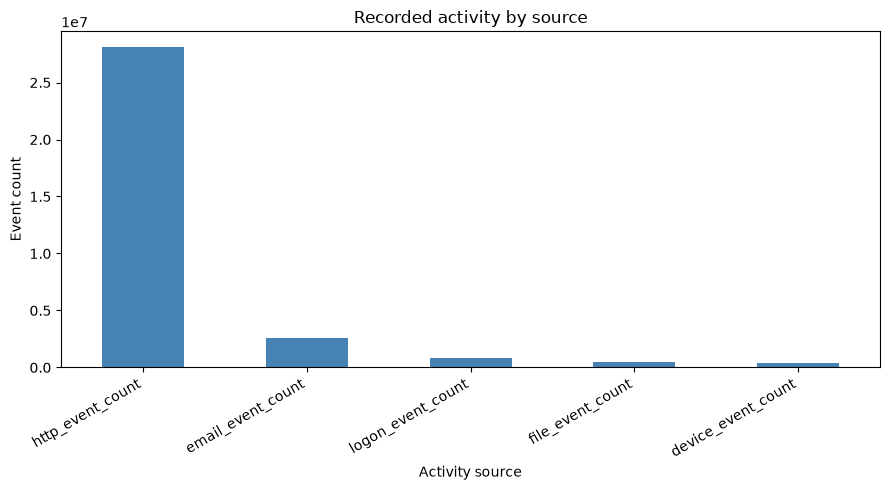
\includegraphics[width=0.9\textwidth]{notebook-1.png}
\caption{Total retained events by source in the saved analysis notebook}
\label{fig:source-events}
\end{figure}

\begin{figure}[H]
\centering
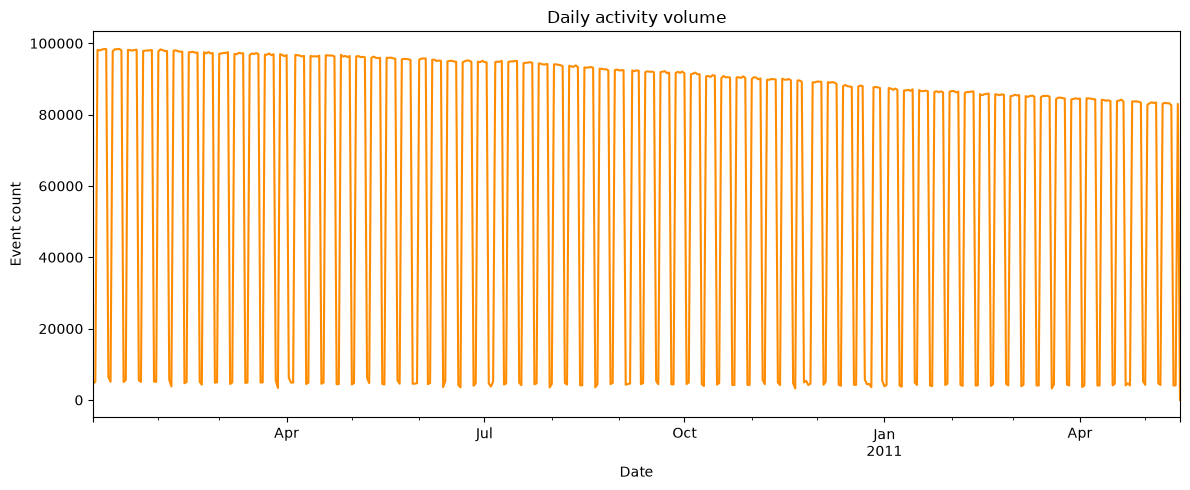
\includegraphics[width=0.95\textwidth]{notebook-2.png}
\caption{Daily recorded activity volume across the dataset period}
\label{fig:daily-events}
\end{figure}

\begin{figure}[H]
\centering
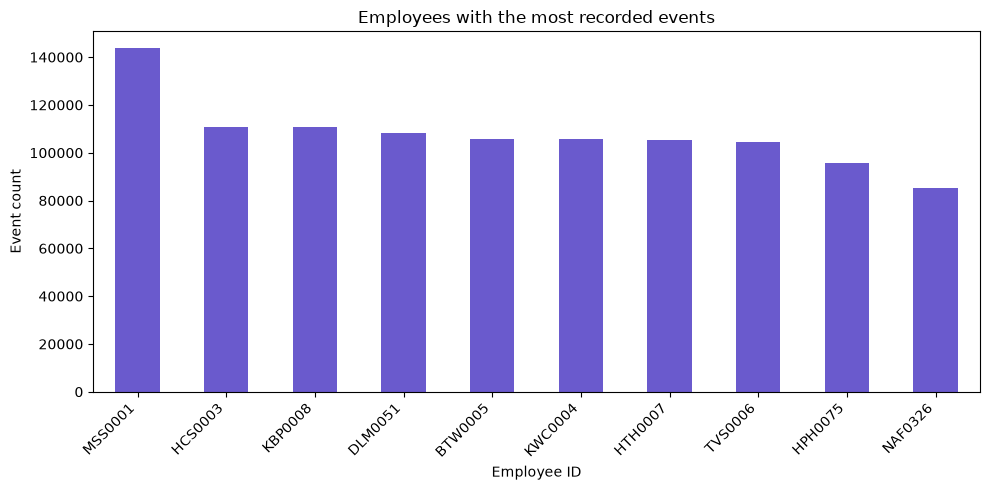
\includegraphics[width=0.95\textwidth]{notebook-3.png}
\caption{Ten synthetic users with the highest aggregate event counts}
\label{fig:user-events}
\end{figure}

The first plot makes the scale imbalance among event sources visible:
HTTP contributes most of the retained rows. The daily plot shows a
recurring low-activity pattern alongside a declining baseline over
time; it is a dataset overview, not evidence that any user is
anomalous. The employee plot is descriptive only and does not adjust
for working days, role, or tenure.

\section{Analysis of architecture and algorithms}
\subsection{Detailed study of proposed algorithms}
\textbf{Logistic Regression:} A supervised baseline with median
imputation, standard scaling, class weighting, and a maximum of 1,000
iterations. The model is fitted on the training partition and outputs
positive-class scores.

\textbf{Decision Tree:} A supervised tree with maximum depth 10,
minimum leaf size 10, and balanced class weights. These constraints
limit tree complexity compared with an unrestricted tree.

\textbf{Random Forest:} A supervised ensemble of 200 trees, minimum leaf
size 5, balanced-sub-sample class weights, and parallel fitting. It
averages tree predictions to produce a positive-class score.

\textbf{Isolation Forest:} An unsupervised anomaly detector with 200
trees, automatic contamination handling, and parallel fitting. The
negative decision function is used so larger values rank as more
unusual. The contamination setting controls the estimator's outlier
decision threshold; the project separately evaluates a validation-
selected one-percent queue and retains five percent as a reference.

\subsection{Step-by-step model workflow}
\begin{enumerate}
  \item Create numeric employee-day features and known-incident labels.
  \item Reserve one employee-grouped partition for final test evaluation.
  \item Split the remaining employees into training and validation groups.
  \item Fit all models on training records only and score validation and
        test records.
  \item Select the best model by validation Average Precision.
  \item Select review capacity by validation F1 from a coarse candidate
        grid, then compare precision and recall on held-out test employees.
        The selected rate is one percent; keep five percent as a
        larger-capacity reference.
  \item Retrain the saved dashboard bundle using the labelled table after
        evaluation. The dashboard's multi-model review scores are not the
        same thing as the single-model test comparison.
\end{enumerate}

\section{Project pipeline}
\begin{figure}[H]
\centering
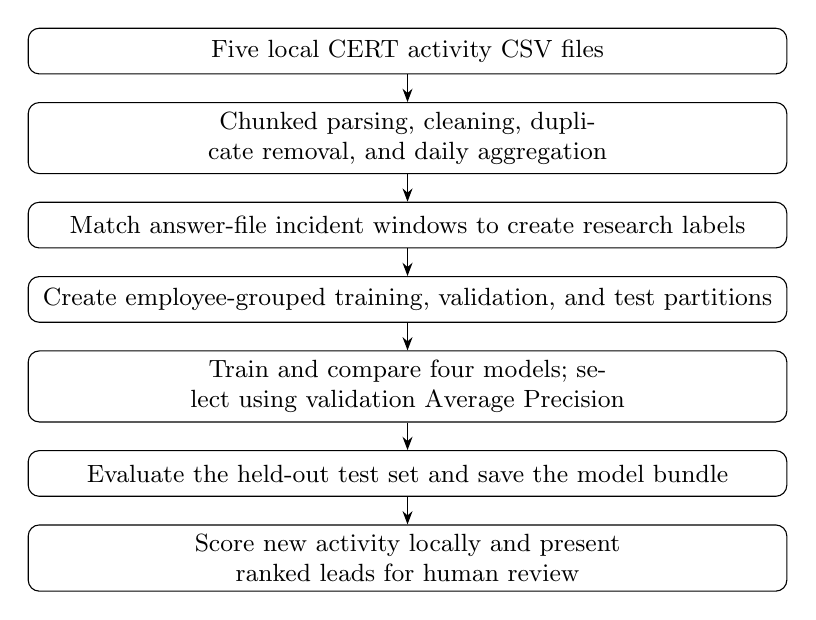
\begin{tikzpicture}[
  stage/.style={draw,rounded corners,align=center,text width=9.4cm,minimum height=0.58cm,font=\small},
  flow/.style={-{Stealth},thin}
]
\node[stage] (sources) {Five local CERT activity CSV files};
\node[stage,below=0.35cm of sources] (clean) {Chunked parsing, cleaning, duplicate removal, and daily aggregation};
\node[stage,below=0.35cm of clean] (label) {Match answer-file incident windows to create research labels};
\node[stage,below=0.35cm of label] (split) {Create employee-grouped training, validation, and test partitions};
\node[stage,below=0.35cm of split] (models) {Train and compare four models; select using validation Average Precision};
\node[stage,below=0.35cm of models] (outputs) {Evaluate the held-out test set and save the model bundle};
\node[stage,below=0.35cm of outputs] (review) {Score new activity locally and present ranked leads for human review};
\draw[flow] (sources) -- (clean);
\draw[flow] (clean) -- (label);
\draw[flow] (label) -- (split);
\draw[flow] (split) -- (models);
\draw[flow] (models) -- (outputs);
\draw[flow] (outputs) -- (review);
\end{tikzpicture}
\caption{High-level project pipeline}
\end{figure}

\section{Feasibility analysis}
\subsection{Technical feasibility}
The analysis pipeline is implemented in Python using pandas, NumPy,
scikit-learn, and joblib. FastAPI serves the local analysis service; the
React client is built with Vite, and Streamlit remains an alternative
interface. Chunked CSV processing makes the main event
ingestion feasible on a developer workstation. The repository includes
the dataset directory locally, while generated outputs are ignored by
Git. The demonstrated environment is macOS on Apple silicon with Python
3.14.8, pandas 3.0.6, NumPy 2.5.3, scikit-learn 1.9.1, FastAPI, and
React. These versions describe the checked environment and are not a
claim of a fully reproducible environment lockfile.

\subsection{Economic feasibility}
The prototype uses free, open-source Python libraries and runs locally.
The main costs are developer time, storage for the raw logs and derived
outputs, and the compute time required to process large CSV files. No
cloud service, paid API, or hosted database is required for the
demonstration. Production costs would additionally include access
controls, auditing, secure retention, model monitoring, and analyst
review capacity.

\subsection{Operational feasibility}
The intended operator is an authorised analyst who can choose a folder
of expected CSVs, run analysis, inspect a ranked queue, and compare model
rank scores with underlying activity days. Operational use would require
documented policies, access authorization, a defined alert capacity,
case notes, independent corroboration, and a process to correct
inaccurate data or interpretations. Those governance systems are not
implemented in this prototype.

\section{System environment}
\subsection{Software environment}
\begin{itemize}
  \item Operating system used for verification: macOS 27.0.1, Apple
        silicon.
  \item Python: 3.14.8.
  \item pandas 3.0.6; NumPy 2.5.3; scikit-learn 1.9.1.
  \item FastAPI and Uvicorn for the local API; React and Vite for the
        primary web client; Streamlit 1.65.0 for the alternative client.
        Joblib persists the estimator bundle.
  \item Jupyter notebook: \texttt{notebook/forensic.ipynb}.
  \item Primary demo entry points: \texttt{api.py} and
        \texttt{frontend/}; alternative entry point:
        \texttt{app.py}.
\end{itemize}

\subsection{Hardware environment}
The checked development environment is a Mac with Apple silicon; the
repository does not record a verified RAM, storage, or processor-core
specification. The program parallelizes selected estimator operations
and processes large source files in chunks. Hardware recommendations
should be established by measuring end-to-end runtime and peak memory
on the target deployment machine rather than inferred from this report.

\section{Actors and roles}
\begin{description}
  \item[Analyst] Selects the activity folder, runs analysis, reviews
        ranked users and their supporting activity-day indicators, and
        validates leads independently.
  \item[Project developer] Maintains preprocessing, model training,
        evaluation, and dashboard code.
  \item[Supervisor / administrator] Authorizes use, controls access to
        sensitive logs, and defines retention and review procedures.
  \item[Model] Computes relative scores from the engineered numeric
        features; it does not make employment or disciplinary decisions.
\end{description}

\section{Functional and non-functional requirements}
The requirements below describe the demonstrated prototype, not a
production insider-risk service. Requirements that concern governance
and operational assurance are stated as constraints because the current
repository does not implement them.

\begin{longtable}{|p{0.09\textwidth}|p{0.52\textwidth}|p{0.34\textwidth}|}
\caption{Functional requirements and implementation evidence}
\label{tab:functional-requirements}\\
\hline
ID & Requirement & Evidence / limitation\\
\hline
\endfirsthead
\hline
ID & Requirement & Evidence / limitation\\
\hline
\endhead
FR01 & Accept the five named activity CSV files from a selected local folder & React folder picker and required-file validation in \texttt{api.py}\\
\hline
FR02 & Read large files incrementally rather than loading each entire source at once & 25,000-row pandas chunks\\
\hline
FR03 & Exclude rows without a usable user or parsed date and remove duplicates within each chunk & Notebook and dashboard preprocessing; cross-chunk duplicates may remain\\
\hline
FR04 & Aggregate retained records by user and calendar day into numeric activity features & Notebook and \texttt{process\_activity\_file()}\\
\hline
FR05 & Align dashboard features to the ordered feature list used at training time & Saved model bundle; missing expected columns are filled with zero\\
\hline
FR06 & Produce comparative model scores and a ranked employee review list & Four estimators and consensus ranking in \texttt{score\_folder()}\\
\hline
FR07 & Show signals and high-ranked activity days supporting a review lead & React interface; signal rules are descriptive, not causal explanations\\
\hline
FR08 & Save review summaries as CSV artifacts & \texttt{dashboard\_report.csv} and \texttt{dashboard\_day\_scores.csv}\\
\hline
\end{longtable}

\begin{longtable}{|p{0.09\textwidth}|p{0.52\textwidth}|p{0.34\textwidth}|}
\caption{Non-functional requirements and current status}
\label{tab:nonfunctional-requirements}\\
\hline
ID & Requirement & Current status\\
\hline
\endfirsthead
\hline
ID & Requirement & Current status\\
\hline
\endhead
NFR01 & Keep the demonstration local and avoid sending activity data to an external service & Implemented for the demonstrated flow\\
\hline
NFR02 & Handle large event files within workstation memory constraints & Chunked input is implemented; peak memory has not been measured\\
\hline
NFR03 & Make outputs understandable and subject to human review & Caution text and activity context are shown; no case-management workflow\\
\hline
NFR04 & Protect raw records and generated outputs from unauthorized access & Not implemented; local permissions remain the operator's responsibility\\
\hline
NFR05 & Record access, analyst decisions, model versions, and retention actions & Not implemented\\
\hline
NFR06 & Demonstrate generalization to operational data and acceptable review burden & Not established by the synthetic, employee-day experiment\\
\hline
\end{longtable}

The requirements highlight the boundary between a working prototype
and a deployable decision-support system. File ingestion and ranking
are present, but access control, auditability, retention, and evidence
management require separate design and validation before operational
use.

\chapter{System Design}
\section{Model(s) Building}
The implementation is divided between the analysis notebook and the
React/FastAPI application. The notebook performs bulk preparation,
incident-window labelling, grouped evaluation, and model serialization.
The application loads the saved feature list and estimator bundle,
rebuilds employee-day features from selected CSV files, and displays
ranked review leads.

\subsection{Implementation code}
The notebook is the source of the training and evaluation workflow.
The primary dashboard uses \texttt{frontend/src/App.jsx} for the React
interface, \texttt{api.py} for its FastAPI endpoints, and
\texttt{forensic\_core.py} for CSV parsing, feature alignment,
four-model scoring, and employee ranking. The Streamlit alternative is
implemented in \texttt{app.py}. Selected source excerpts are included in
the appendix; the full source files remain in the project repository.

\subsection{Model planning and training/testing split}
The labelled employee-day records are separated by employee identifier,
not by randomly splitting individual days. This keeps one synthetic
employee's records within a single partition and reduces leakage from
repeated observations of the same employee. The training partition is
used to fit the estimators; the validation partition is used to select a
model by Average Precision; the test partition is reserved for final
comparison. Partition sizes and positive-label counts are reported in
Chapter~\ref{chap:results}.

\subsection{Training}
Logistic Regression, Decision Tree, Random Forest, and Isolation Forest
are fitted using the configured preprocessing and estimator settings
described in the system-analysis chapter. The first three use the
training labels; Isolation Forest is fitted as an unsupervised anomaly
detector without those labels. The notebook stores the model objects,
their names, and ordered feature columns in a joblib bundle for the
dashboard.

\subsection{Testing}
The held-out employee groups are scored after training. Supervised
scores use the positive-class output; Isolation Forest scores are
direction-adjusted so larger values correspond to more unusual
observations. Model selection and the test metrics are kept distinct.
The saved comparison and confusion-matrix counts are detailed in
Chapter~\ref{chap:results}; the test-set results do not validate the
dashboard's separate employee-level consensus rule.

\section{System Design Diagrams}
\subsection{Use-case model}
\begin{figure}[H]
\centering
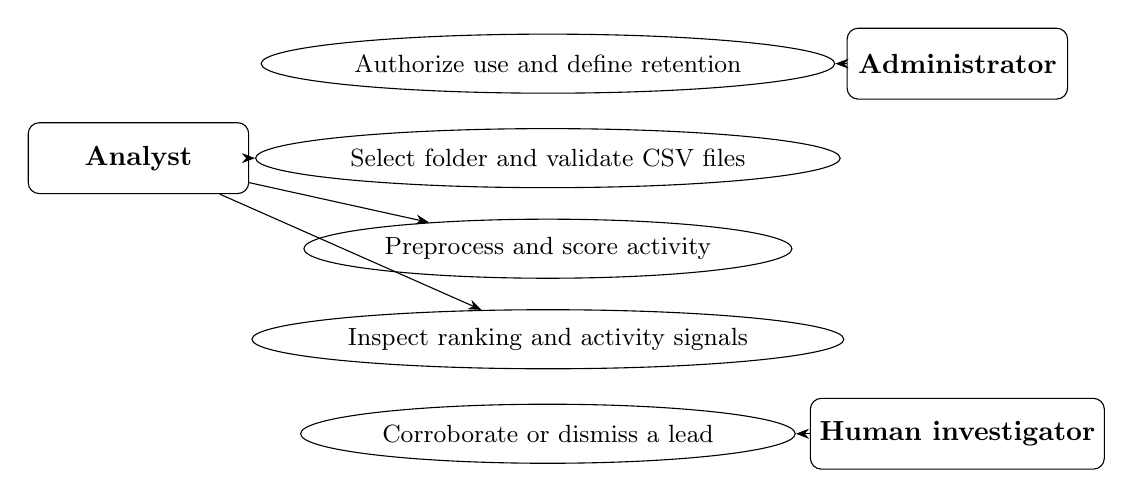
\begin{tikzpicture}[
  usecase/.style={draw,ellipse,align=center,minimum width=4.1cm,minimum height=0.75cm,font=\small},
  actor/.style={draw,rounded corners,align=center,minimum width=2.8cm,minimum height=0.9cm,font=\normalsize\bfseries},
  link/.style={-{Stealth},thin}
]
\node[actor] (analyst) at (-5.2,0) {Analyst};
\node[actor] (admin) at (5.2,1.2) {Administrator};
\node[actor] (reviewer) at (5.2,-3.5) {Human investigator};
\node[usecase] (select) at (0,0) {Select folder and validate CSV files};
\node[usecase] (score) at (0,-1.15) {Preprocess and score activity};
\node[usecase] (inspect) at (0,-2.3) {Inspect ranking and activity signals};
\node[usecase] (review) at (0,-3.5) {Corroborate or dismiss a lead};
\node[usecase] (govern) at (0,1.2) {Authorize use and define retention};
\draw[link] (analyst) -- (select);
\draw[link] (analyst) -- (score);
\draw[link] (analyst) -- (inspect);
\draw[link] (admin.west) -- (govern.east);
\draw[link] (reviewer) -- (review);
\end{tikzpicture}
\caption{Use-case model for the prototype}
\end{figure}

\subsection{Activity diagram}
\begin{figure}[H]
\centering
\begin{tikzpicture}[
  step/.style={draw,rounded corners,align=center,text width=8.0cm,minimum height=0.58cm,font=\small},
  decision/.style={draw,diamond,aspect=3,align=center,text width=3.2cm,minimum height=0.8cm,font=\small},
  flow/.style={-{Stealth},thin}
]
\node[step] (start) {Start and load the saved model bundle};
\node[step,below=0.42cm of start] (folder) {Choose the folder containing the five activity CSV files};
\node[decision,below=0.5cm of folder] (valid) {Are all required files present?};
\node[step,below=0.62cm of valid] (parse) {Read in chunks, clean rows, and aggregate employee-days};
\node[step,below=0.42cm of parse] (score) {Align features, score with four models, and rank employees};
\node[step,below=0.42cm of score] (review) {Display review leads; analyst checks original logs and context};
\node[step,right=1.1cm of valid,text width=2.5cm] (error) {Show missing-file error and stop};
\draw[flow] (start) -- (folder);
\draw[flow] (folder) -- (valid);
\draw[flow] (valid) -- node[right,font=\scriptsize]{Yes} (parse);
\draw[flow] (parse) -- (score);
\draw[flow] (score) -- (review);
\draw[flow] (valid) -- node[above,font=\scriptsize]{No} (error);
\end{tikzpicture}
\caption{Activity flow for one dashboard review}
\end{figure}

\subsection{Sequence diagram}
\begin{figure}[H]
\centering
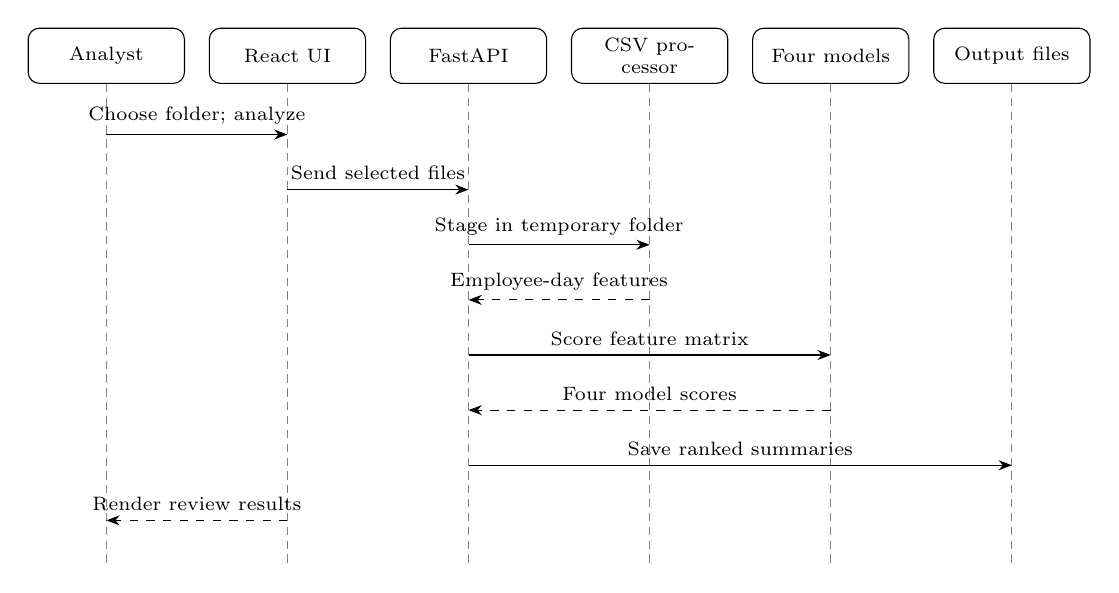
\begin{tikzpicture}[
  participant/.style={draw,rounded corners,align=center,text width=1.75cm,minimum height=0.7cm,font=\scriptsize},
  message/.style={-{Stealth},thin},
  return/.style={-{Stealth},thin,dashed}
]
\node[participant] (user) at (0,0) {Analyst};
\node[participant] (ui) at (2.3,0) {React UI};
\node[participant] (api) at (4.6,0) {FastAPI};
\node[participant] (csv) at (6.9,0) {CSV processor};
\node[participant] (model) at (9.2,0) {Four models};
\node[participant] (store) at (11.5,0) {Output files};
\foreach \x in {user,ui,api,csv,model,store}
  \draw[densely dashed,gray] (\x.south) -- ++(0,-6.1);
\draw[message] (0,-1.0) -- node[above,font=\scriptsize]{Choose folder; analyze} (2.3,-1.0);
\draw[message] (2.3,-1.7) -- node[above,font=\scriptsize]{Send selected files} (4.6,-1.7);
\draw[message] (4.6,-2.4) -- node[above,font=\scriptsize]{Stage in temporary folder} (6.9,-2.4);
\draw[return] (6.9,-3.1) -- node[above,font=\scriptsize]{Employee-day features} (4.6,-3.1);
\draw[message] (4.6,-3.8) -- node[above,font=\scriptsize]{Score feature matrix} (9.2,-3.8);
\draw[return] (9.2,-4.5) -- node[above,font=\scriptsize]{Four model scores} (4.6,-4.5);
\draw[message] (4.6,-5.2) -- node[above,font=\scriptsize]{Save ranked summaries} (11.5,-5.2);
\draw[return] (2.3,-5.9) -- node[above,font=\scriptsize]{Render review results} (0,-5.9);
\end{tikzpicture}
\caption{Sequence of an analysis request}
\end{figure}

\subsection{Class and component design}
\begin{figure}[H]
\centering
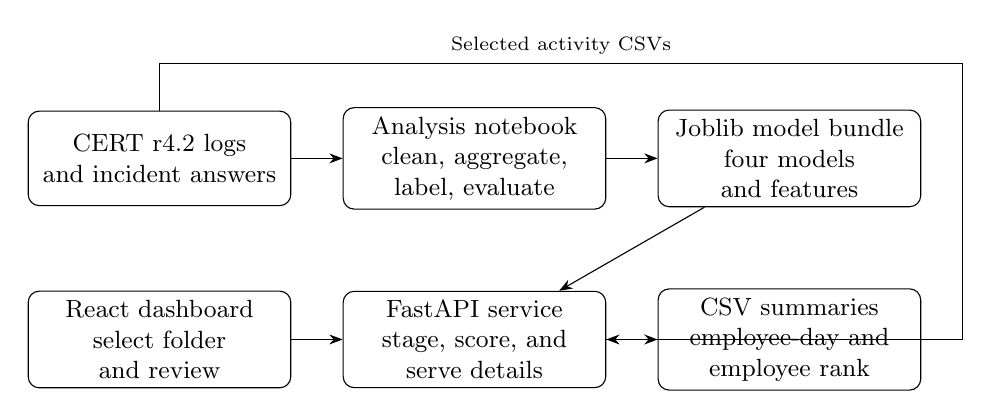
\begin{tikzpicture}[
  component/.style={draw,rounded corners,align=center,text width=3.1cm,minimum height=1.2cm,font=\small},
  flow/.style={-{Stealth},thin}
]
\node[component] (data) at (0,0) {CERT r4.2 logs\\and incident answers};
\node[component] (notebook) at (4,0) {Analysis notebook\\clean, aggregate, label, evaluate};
\node[component] (bundle) at (8,0) {Joblib model bundle\\four models and features};
\node[component] (ui) at (0,-2.3) {React dashboard\\select folder and review};
\node[component] (api) at (4,-2.3) {FastAPI service\\stage, score, and serve details};
\node[component] (outputs) at (8,-2.3) {CSV summaries\\employee-day and employee rank};
\draw[flow] (data) -- (notebook);
\draw[flow] (notebook) -- (bundle);
\draw[flow] (bundle) -- (api);
\draw[flow] (ui) -- (api);
\draw[flow] (api) -- (outputs);
\draw[flow] (data.north) -- (0,1.2)
  -- node[above,font=\scriptsize]{Selected activity CSVs} (10.2,1.2)
  -- (10.2,-2.3) -- (api.east);
\end{tikzpicture}
\caption{Logical component view of the project}
\end{figure}

\section{Project pipeline and output design}
The training notebook writes a model bundle containing the estimator
dictionary, feature names, and model names. The FastAPI service loads
this bundle, creates the same daily numeric feature columns from
the five input sources, fills absent columns with zero, and calculates
four model scores. Scores are converted to within-dataset percentile
ranks and averaged for a consensus employee ranking. The dashboard
marks the top five percent of users by consensus and users in the top
ten percent for at least two models as ``SUSPICIOUS''; remaining users
are marked ``REVIEW''. These are application-specific review labels,
not validated probability thresholds.

Generated CSV reports are saved under \texttt{sprint1\_output}. There is
no database in the current implementation. CSV and joblib files are
local artifacts, so file permissions, encryption, backup, and deletion
must be managed by the operator.

\section{Database design}
No relational database is implemented. The logical data entities are:
\textbf{ActivityEvent} (source row), \textbf{EmployeeDay} (user, day,
feature counts, target label for evaluation), \textbf{ModelArtifact}
(model names and feature columns), \textbf{EmployeeRanking} (user,
relative scores, review status), and \textbf{ReviewSignal} (reason and
supporting high-ranked activity day). CSV is used for tabular
interchange, and joblib serializes Python estimators. A production
version should define explicit schemas, provenance, retention controls,
and access logs before introducing persistent case data.

\section{UI design}
The primary interface is a React dashboard served locally by Vite and
connected to a FastAPI service on the same computer. The landing view
includes the activity-folder picker, model names, a human-review
caution, and an expandable guide that shows how the five activity
sources become employee-day features, pass through four independent
models, and become a percentile-ranked queue. The guide explains the
distinct roles of Isolation Forest, Logistic Regression, Decision Tree,
and Random Forest. After analysis, the dashboard presents summary
counts, prioritized review cards, a searchable and filterable employee
directory, model-agreement signals, relative model ranks, and each
selected employee's highest-ranked activity days. Explanations use
aggregated counts and timing signals rather than message bodies, URLs,
or file contents. The visual design uses a dark navy sidebar, cool
neutral surfaces, and distinct restrained accents for the four model
views. The selected CSV files are sent to the local API,
staged in a temporary folder, and removed from that staging folder after
analysis; the generated dashboard summaries are saved under
\texttt{sprint1\_output}. The previous Streamlit interface remains
available as an alternative.

\begin{figure}[H]
\centering
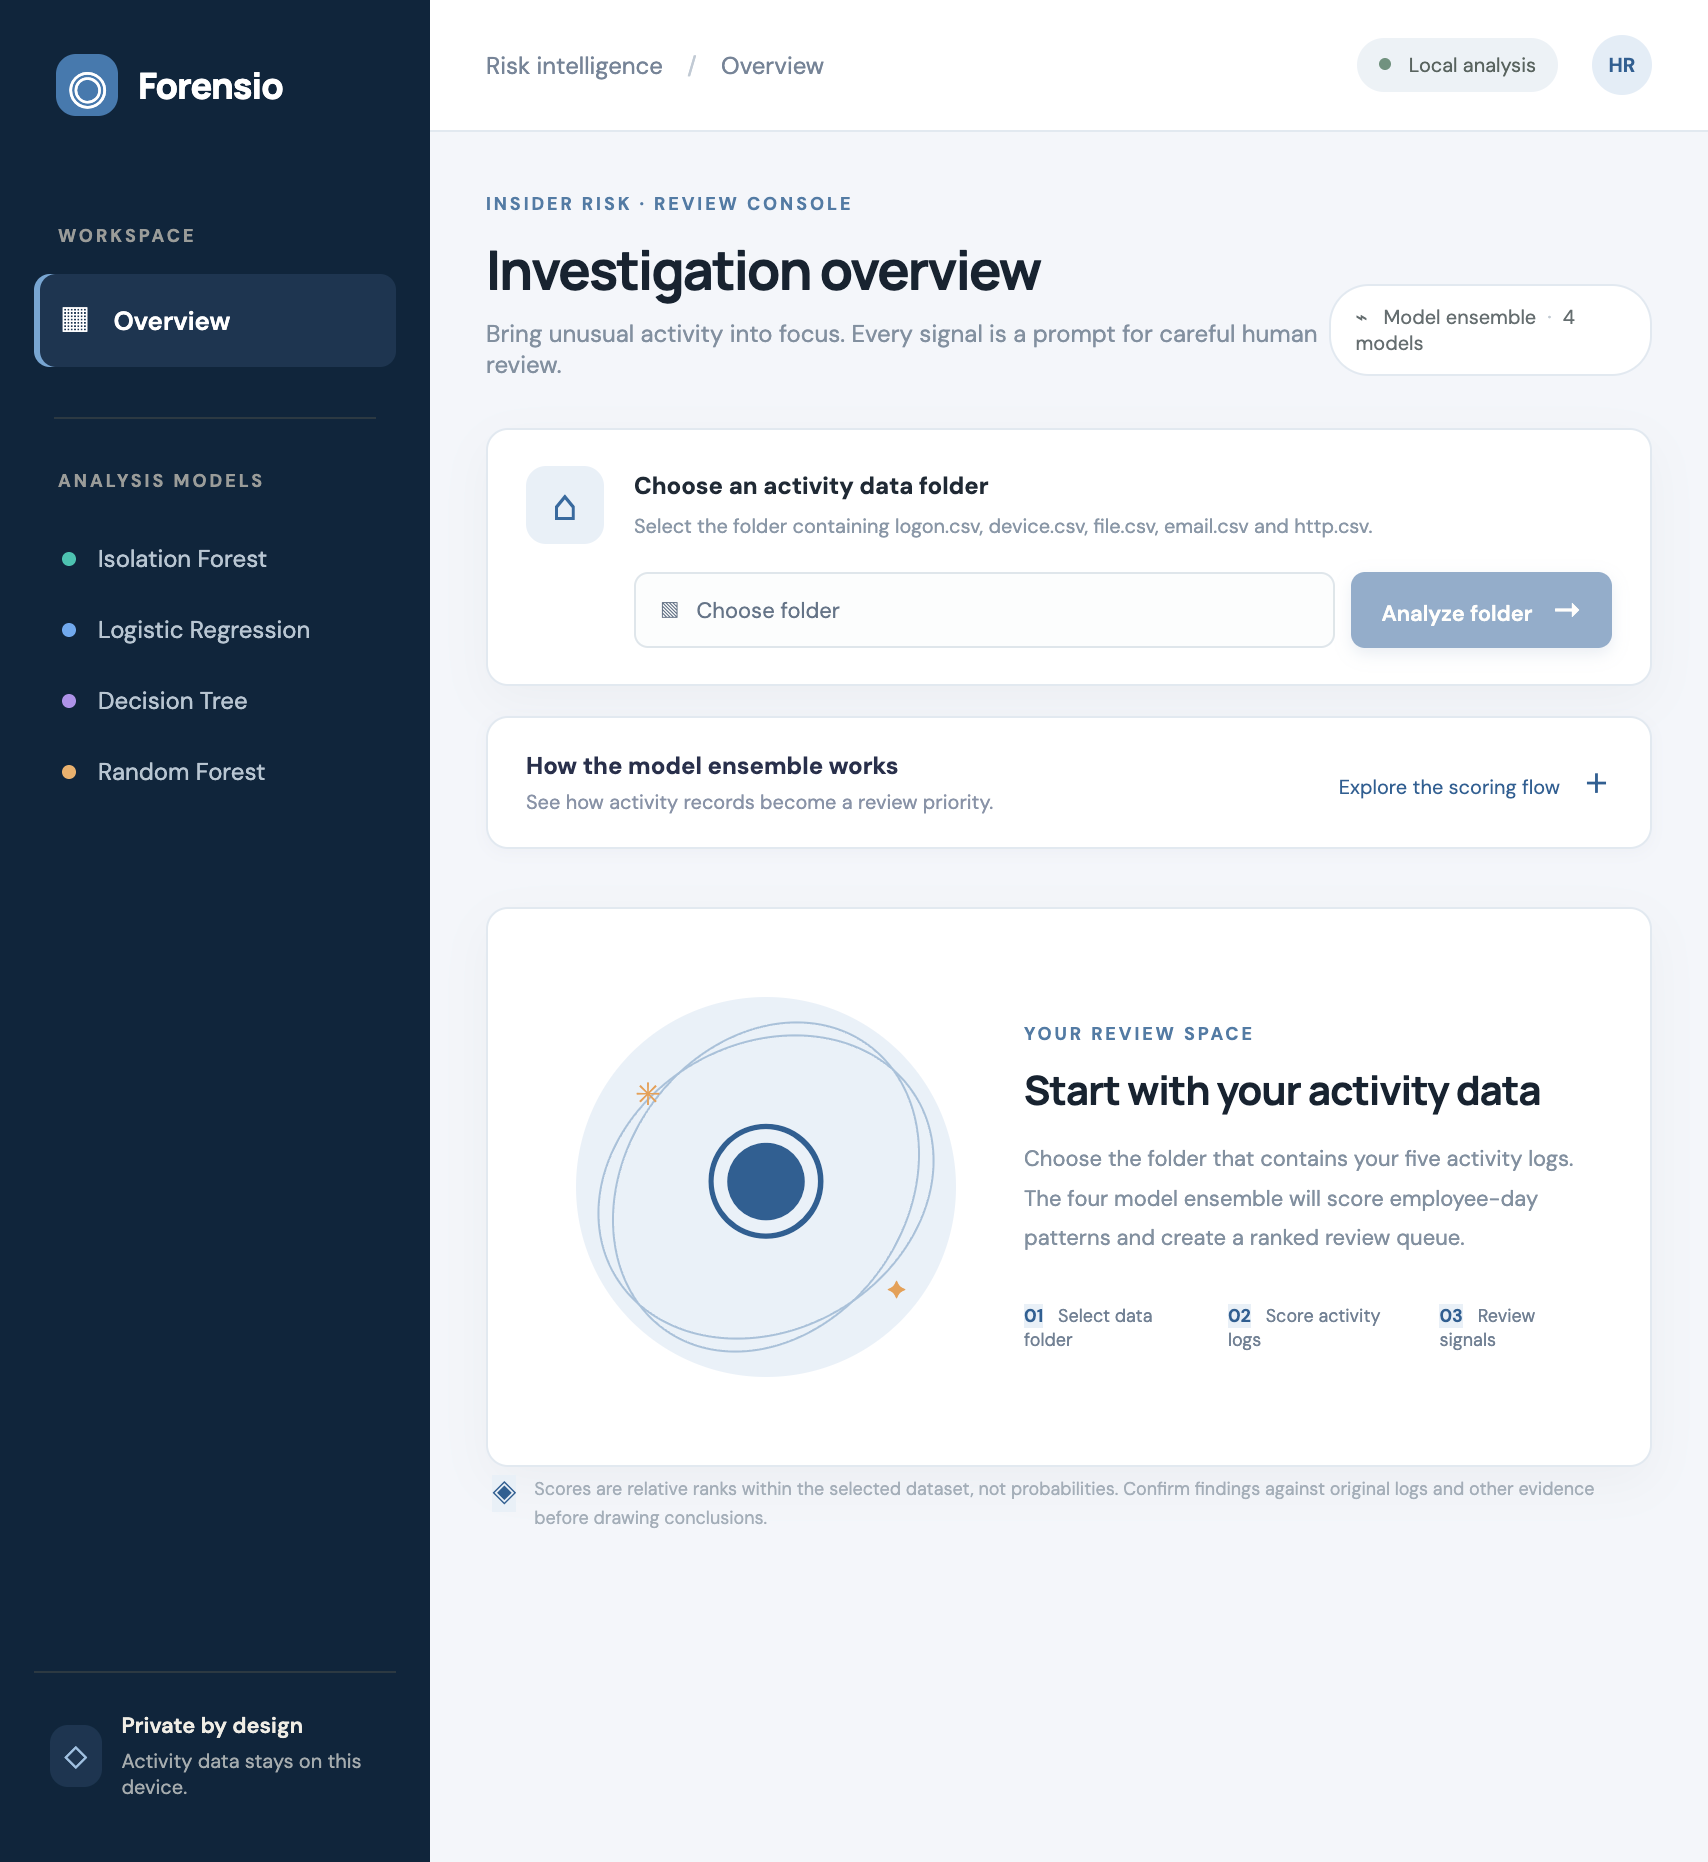
\includegraphics[height=0.50\textheight,keepaspectratio]{ui_react_landing.png}
\caption{React dashboard before an activity folder is selected; the local model service is available.}
\label{fig:dashboard-landing}
\end{figure}

\begin{figure}[H]
\centering
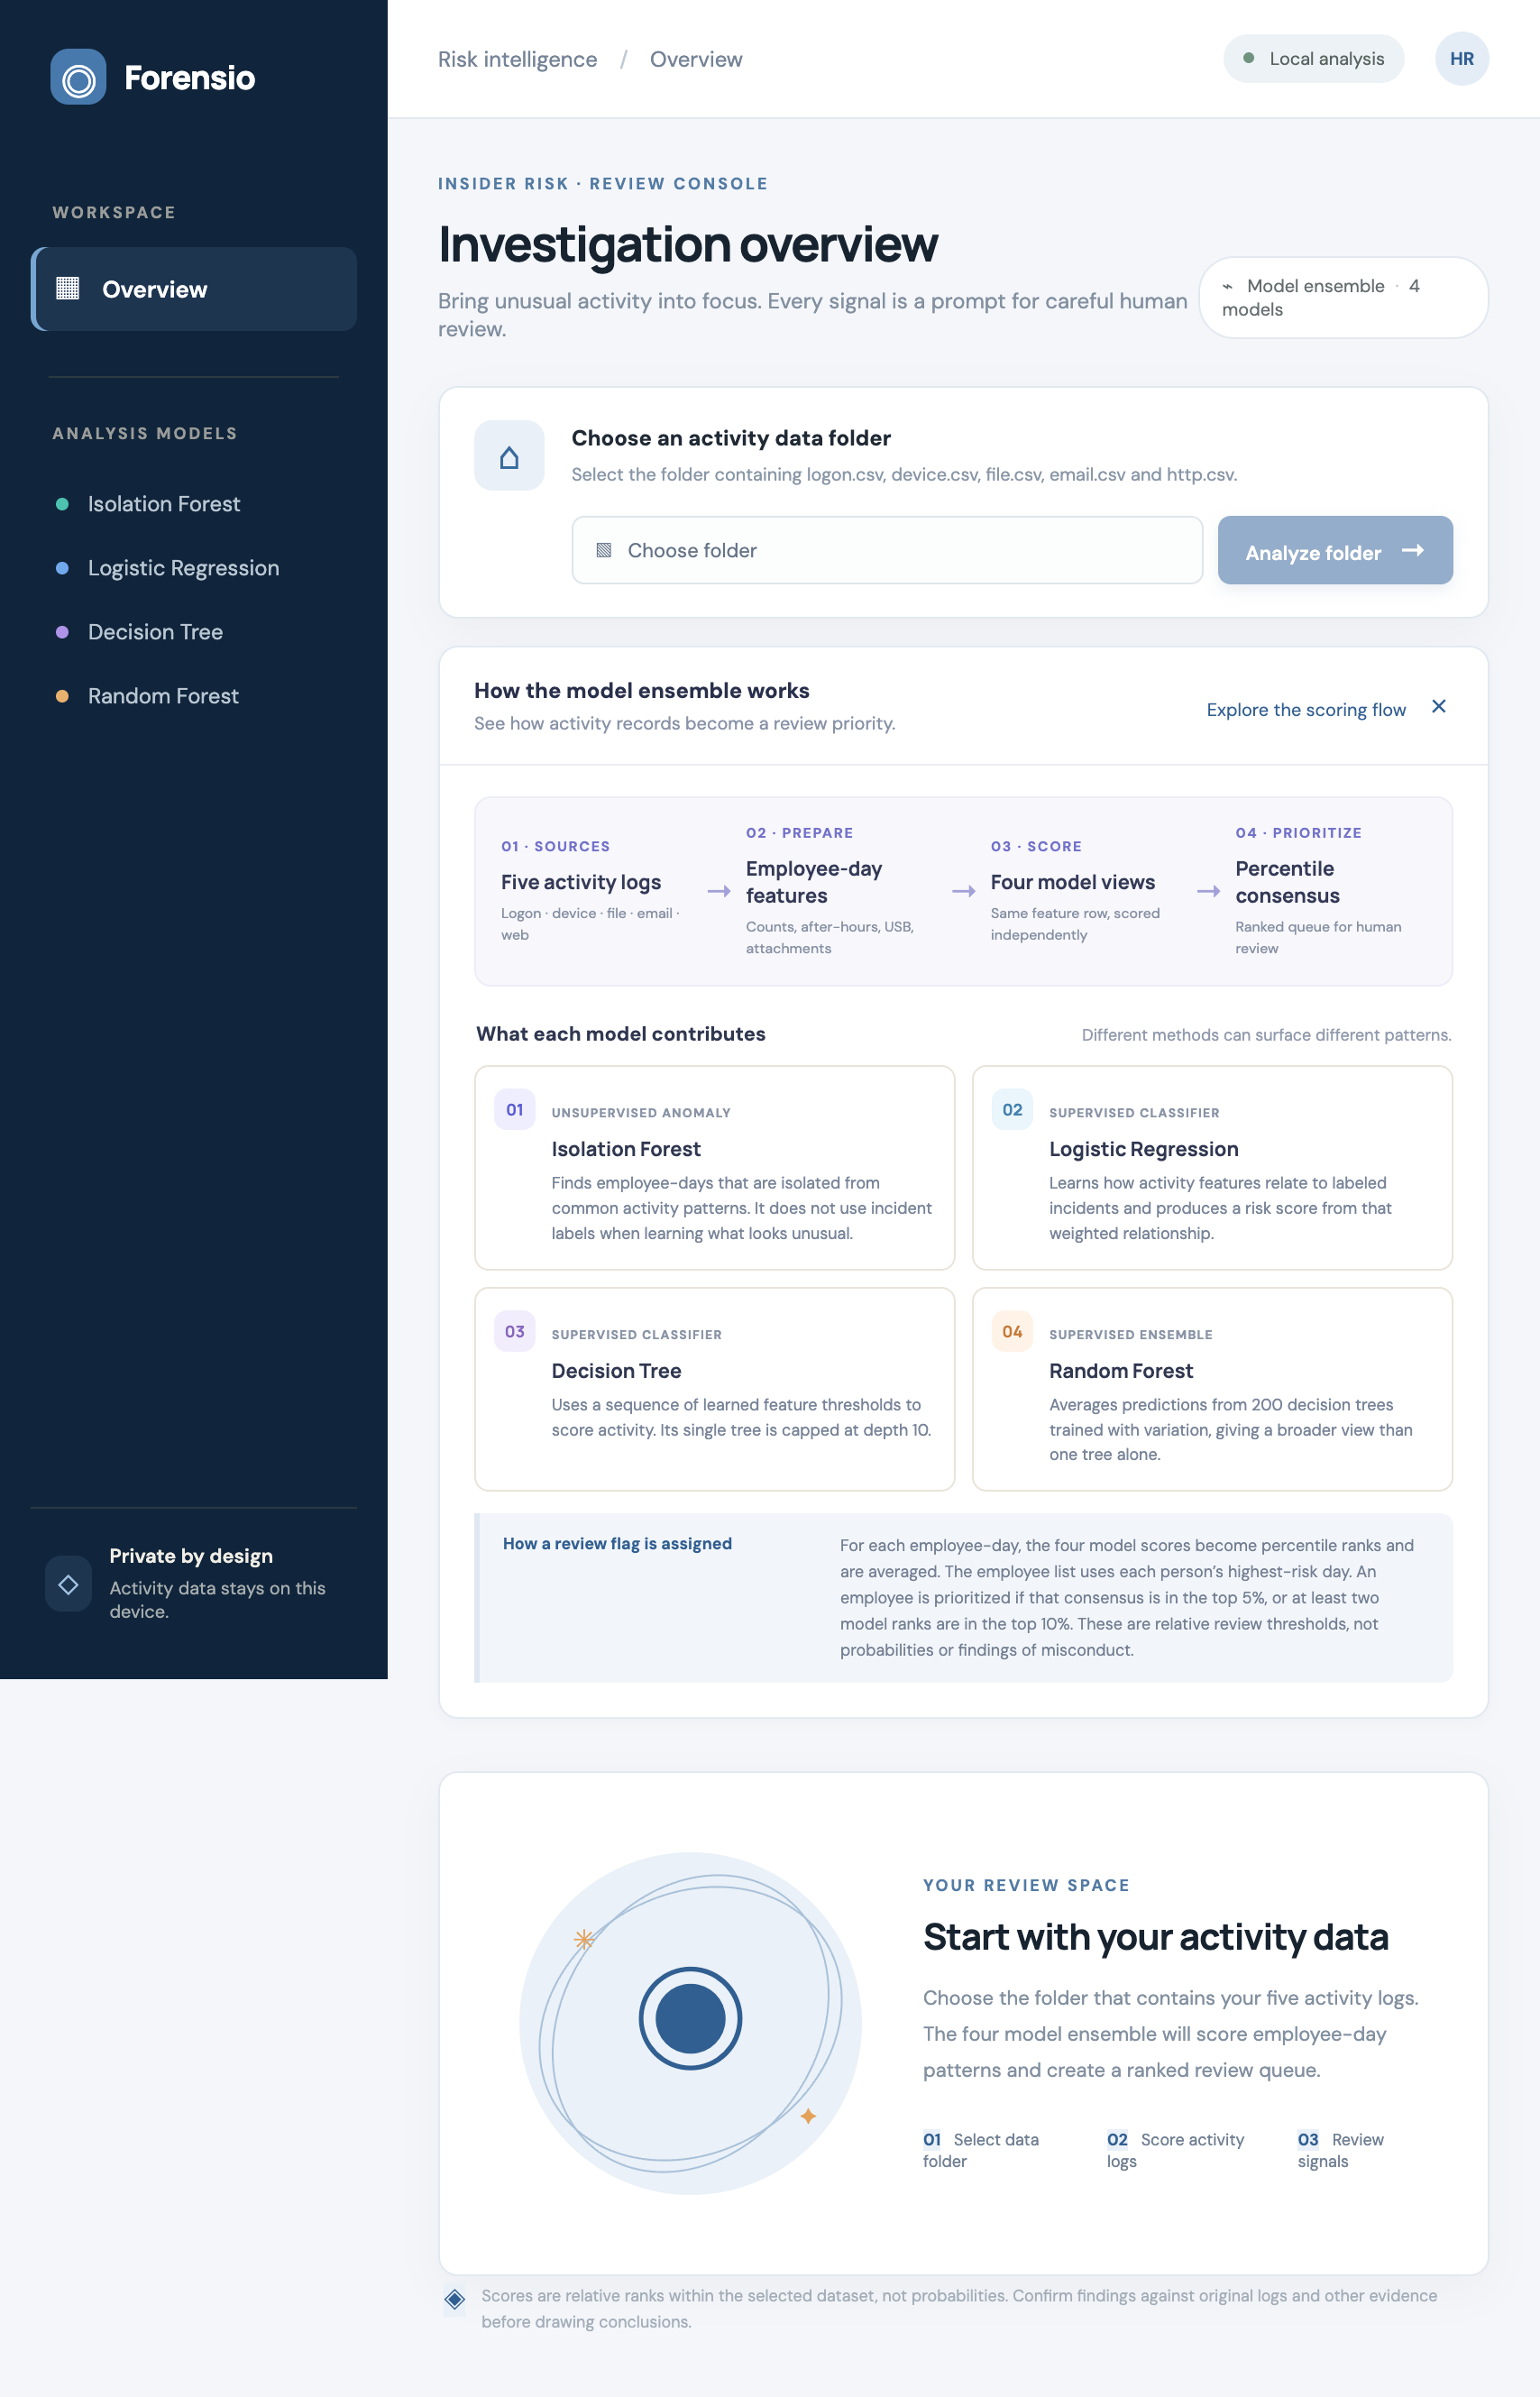
\includegraphics[height=0.66\textheight,keepaspectratio]{ui_react_model_guide.png}
\caption{Expanded guide from the React dashboard, showing the activity-to-review flow, each model's role, and the live employee-level review rule.}
\label{fig:dashboard-model-guide}
\end{figure}

\chapter{Results and Discussion}
\label{chap:results}
\section{Testing approach}
The repository contains no dedicated automated test suite. Verification
for this report consisted of reading the actual source and saved
artifacts, checking the saved schema and quality summaries, running the
grouped split and model evaluation against the saved labelled CSV, and
checking Python syntax for notebook code cells. The dashboard was not
subjected to a documented end-to-end analyst acceptance test in this
report. The React landing screen and expanded model guide were captured
while the local API reported the model bundle as ready; no folder
analysis was run for those screenshots. Table~\ref{tab:tests}
distinguishes completed checks from recommended manual tests.

\begin{longtable}{|p{0.09\textwidth}|p{0.55\textwidth}|p{0.31\textwidth}|}
\caption{Test cases and verification status}
\label{tab:tests}\\
\hline
ID & Test / expected behavior & Status\\
\hline
\endfirsthead
\hline
ID & Test / expected behavior & Status\\
\hline
\endhead
T01 & Parse all notebook code cells; no syntax errors & Passed\\
\hline
T02 & Verify saved labelled table dimensions, users, date span, and positive count & Passed\\
\hline
T03 & Verify grouped train/validation/test partitions have positive labels and no user overlap & Passed\\
\hline
T04 & Refit the four configured estimators and calculate validation/test metrics on saved data & Passed\\
\hline
T05 & Confirm test predictions and confusion-matrix totals at the validation-selected capacity & Passed\\
\hline
T06 & Select a folder missing a required CSV; application should display a clear error & Recommended manual test\\
\hline
T07 & Analyze a valid folder and compare dashboard feature totals with notebook output & Recommended manual test\\
\hline
T08 & Test malformed dates, blank users, duplicate rows across chunk boundaries, and empty files & Recommended automated tests\\
\hline
T09 & Verify output permissions and deletion/retention for sensitive logs & Not implemented\\
\hline
\end{longtable}

\section{Model planning and evaluation protocol}
The saved evaluation artifact records ranking and fixed-capacity
metrics. Average Precision selects the model. A review rate is selected
by validation F1 for that model from the candidate capacities 1\%, 2\%,
3\%, 5\%, 7.5\%, 10\%, 15\%, and 20\%; test data is not used to choose
the rate. Test metrics are reported after the model and operating
capacity are fixed. The saved split groups records by user and contains
198,259 training
rows with 815 positive labels, 66,075 validation rows with 260 positive
labels, and 66,118 test rows with 289 positive labels. The three user
sets are disjoint.

For each partition, scores are sorted to select the chosen proportion.
This is a ranking-based operating point, not a fixed score threshold.
The selected one-percent test queue contains 662 employee-days; the
five-percent comparison queue contains 3,306. Metrics are rounded in
the tables, so counts from the confusion matrices are authoritative.

\section{Comparison of models}
At the validation-selected one-percent review capacity, the results are:
\begin{table}[H]
\centering
\caption{Metrics at the 1\% queue rate selected by validation F1}
\label{tab:selected-capacity}
\small
\begin{tabularx}{\textwidth}{|>{\raggedright\arraybackslash}p{0.20\textwidth}|*{5}{>{\centering\arraybackslash}X|}}
\hline
Model & Validation F1 & Test P@1\% & Test R@1\% & Test F1 & Test AP\\
\hline
Random Forest & 0.235 & 0.094 & 0.215 & 0.130 & 0.088\\
\hline
Decision Tree & 0.185 & 0.121 & 0.277 & 0.168 & 0.104\\
\hline
Logistic Regression & 0.011 & 0.003 & 0.007 & 0.004 & 0.027\\
\hline
Isolation Forest & 0.015 & 0.027 & 0.062 & 0.038 & 0.027\\
\hline
\end{tabularx}
\end{table}

Random Forest remains selected because it has the highest validation AP
(0.214). The one-percent rate is the best F1 among the predeclared
validation capacities for that model. On the held-out test split, its F1
increases from 0.091 at five percent to 0.130 at one percent; recall
falls from 56.40\% to 21.45\%, while precision rises from 4.93\% to
9.37\%. Average Precision is unchanged by the queue cutoff. Decision
Tree's higher test F1 is reported for comparison only and is not used to
select the model or capacity.

The original five-percent results remain useful as a larger-capacity
reference:
\begin{table}[H]
\centering
\caption{Model evaluation from saved \texttt{model\_comparison.csv}}
\label{tab:comparison}
\small
\begin{tabularx}{\textwidth}{|>{\raggedright\arraybackslash}p{0.19\textwidth}|*{5}{>{\centering\arraybackslash}X|}}
\hline
Model & \shortstack{Validation\\AP} & \shortstack{Validation\\P@5\%} & \shortstack{Validation\\R@5\%} & \shortstack{Test\\P@5\%} & \shortstack{Test\\R@5\%}\\
\hline
Random Forest & 0.214 & 0.054 & 0.681 & 0.049 & 0.564\\
\hline
Decision Tree & 0.185 & 0.055 & 0.704 & 0.035 & 0.405\\
\hline
Logistic Regression & 0.027 & 0.037 & 0.465 & 0.037 & 0.419\\
\hline
Isolation Forest & 0.016 & 0.008 & 0.096 & 0.018 & 0.208\\
\hline
\end{tabularx}
\end{table}

\begin{table}[H]
\centering
\caption{Additional test metrics from saved evaluation}
\label{tab:testextra}
\begin{tabularx}{\textwidth}{|l|*{3}{>{\centering\arraybackslash}X|}}
\hline
Model & Test AP & Test F1 @ 5\% & Test accuracy @ 5\%\\
\hline
Random Forest & 0.088 & 0.091 & 0.951\\
\hline
Decision Tree & 0.104 & 0.065 & 0.949\\
\hline
Logistic Regression & 0.027 & 0.067 & 0.949\\
\hline
Isolation Forest & 0.027 & 0.033 & 0.947\\
\hline
\end{tabularx}
\end{table}

Random Forest was selected by the highest validation Average Precision
(0.214). Decision Tree had the highest test Average Precision (0.104),
but choosing a model after inspecting test results would use the held-out
test to tune the selection. The report therefore retains Random Forest
as the validation-selected model and treats test AP as an estimate, not
as another selection criterion. The queue rate is also selected on the
validation partition only; test AP does not change when the review rate
changes.

\section{Evaluation metrics}
\textbf{Precision at 5\%} is the fraction of the fixed-size top-ranked
queue matching known positive labels. \textbf{Recall at 5\%} is the
fraction of all known positive test employee-days found in that queue.
\textbf{Average Precision (AP)} measures ranking performance across
possible score thresholds. \textbf{F1} combines positive-class precision
and recall at the selected queue rule. \textbf{Accuracy} is the fraction
of all test employee-days correctly classified at that same rule. Since
only 289 of 66,118 test records are labelled positive (0.437\%), accuracy
and weighted averages can look strong even when positive-class
precision is low. Macro average gives equal weight to class-level scores
but should not replace inspection of each class.

For a selected queue size \(k\), let \(Q_k\) be the set of the \(k\)
highest-scored test employee-days and let \(P\) be the set of all
employee-days labelled as overlapping a known incident window. The
reported capacity metrics are:
\[
\operatorname{Precision@}k = \frac{|Q_k \cap P|}{k},
\qquad
\operatorname{Recall@}k = \frac{|Q_k \cap P|}{|P|}.
\]
For the capacity-reference results, \(k=\lceil 0.05N\rceil\). The
validation-selected operating point instead uses \(k=\lceil 0.01N\rceil\).
These definitions make the review-capacity assumption explicit:
increasing \(k\) increases the number of records presented for review
and can change both precision and recall. Both rates are recalculated
within each partition and should not be mistaken for transferable
probability thresholds.

For the dashboard, let \(r_{u,d,m}\) be model \(m\)'s percentile rank
for user \(u\) on day \(d\). The interface averages the four model
percentile ranks for each employee-day and then uses that employee's
maximum daily consensus value for its employee ranking:
\[
c_{u,d} = \frac{1}{4}\sum_{m=1}^{4} r_{u,d,m},
\qquad
C_u = \max_d c_{u,d}.
\]
This is an application ranking rule, not a calibrated probability and
not the model-selection rule used in the offline evaluation. The
dashboard also uses a top-five-percent consensus cutoff and a
two-of-four model-agreement condition for its ``SUSPICIOUS'' display
status; those employee-level rules have not been evaluated by the
employee-day test metrics in this report.

\section{Confusion matrix}
\begin{table}[H]
\centering
\caption{Random Forest confusion matrix at the validation-selected 1\% queue rate}
\label{tab:matrix}
\begin{tabularx}{\textwidth}{|p{0.28\textwidth}|*{2}{>{\centering\arraybackslash}X|}}
\hline
 & \shortstack{Predicted\\not listed} & \shortstack{Predicted\\in known window}\\
\hline
Actual not listed & 65,229 & 600\\
\hline
Actual in known window & 227 & 62\\
\hline
\end{tabularx}
\end{table}

Figure~\ref{fig:threshold-matrices} reproduces the notebook's earlier
five-percent reference confusion matrices. The integer counts in
Table~\ref{tab:matrix} and Appendix~\ref{app:test-counts} show the
validation-selected one-percent operating point.

\begin{figure}[H]
\centering
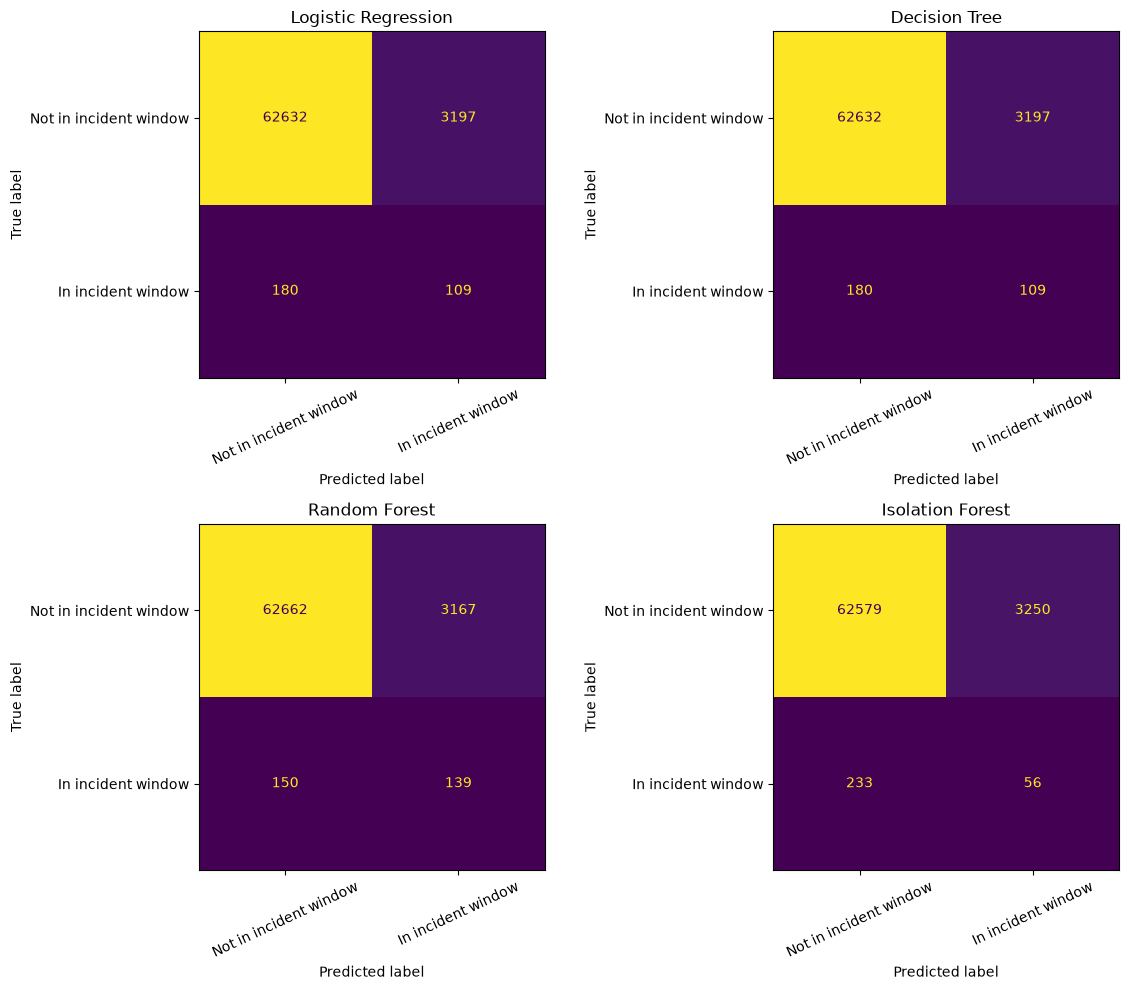
\includegraphics[width=\textwidth]{notebook-4.png}
\caption{Previously saved notebook confusion matrices at the 5\% reference capacity}
\label{fig:threshold-matrices}
\end{figure}

At the selected one-percent capacity, the Random Forest places 62 known
positive employee-days in the 662-record queue and leaves 227 known
positives outside it. The other 600 records do not match a known label;
they are not proven benign. At the five-percent reference capacity, the
model places 163 known positives in 3,306 records and leaves 126 known
positives outside. The lower-capacity option improves test F1 in this
synthetic experiment while retrieving fewer known positives overall.

\section{Discussion}
The model comparison illustrates that unsupervised anomaly detection
does not necessarily rank known incident examples well: Isolation Forest
has test recall 20.8\% and precision 1.8\% at the same queue size. The
supervised Random Forest catches more known positives in the saved test
partition, but its 4.9\% precision means the queue is still dominated by
records without a matching known label. The Decision Tree has a higher
test AP than Random Forest, but its validation AP is lower and its test
recall at the five-percent reference capacity is 40.5\%. This difference emphasizes why
validation-based selection and a one-time test evaluation should be
kept separate.

The experiment evaluates employee-days, while the dashboard ultimately
aggregates scores to rank employees. Employee-level review performance
is not established by the employee-day table. The dashboard also uses
four-model agreement and consensus ranks; those rules are not evaluated
by the reported classification metrics. Additional employee-level and
temporal validation is necessary before making claims about dashboard
effectiveness.

\section{Requirements traceability}
\begin{table}[H]
\centering
\caption{Requirements traceability}
\label{tab:req}
\small
\begin{tabularx}{\textwidth}{|p{0.08\textwidth}|p{0.52\textwidth}|X|}
\hline
ID & Requirement & Implementation / evidence\\
\hline
R01 & Read five activity sources & React folder picker and \texttt{api.py}; notebook ingestion\\
\hline
R02 & Create employee-day numeric features & notebook and \texttt{process\_activity\_file}\\
\hline
R03 & Keep answer labels out of inference upload & answer file used in notebook only\\
\hline
R04 & Compare four models & saved comparison table and bundle\\
\hline
R05 & Hold user groups apart in evaluation & nested grouped train/validation/test split\\
\hline
R06 & Present human-review context & React report, activity indicators, model guide, and caution text\\
\hline
R07 & Establish real-world validity and operational threshold & Not satisfied; future work\\
\hline
\end{tabularx}
\end{table}

\chapter{Model Deployment}
\section{Local demonstration setup}
The primary React demonstration uses two local processes. Start the API
from the project root after installing the Python requirements if needed:
\begin{lstlisting}
./.forensic/bin/python -m pip install -r requirements.txt
./.forensic/bin/python -m uvicorn api:app --host 127.0.0.1 --port 8000
\end{lstlisting}
Then start the web client in a second terminal:
\begin{lstlisting}
cd frontend
npm install
npm run dev
\end{lstlisting}
The model bundle is expected at
\texttt{sprint1\_output/insider\_investigation\_model.joblib}. The user
opens the Vite URL (normally \texttt{http://127.0.0.1:5173}), selects
the folder containing \texttt{logon.csv}, \texttt{device.csv},
\texttt{file.csv}, \texttt{email.csv}, and \texttt{http.csv}, then
selects ``Analyze folder''. The browser sends the selected CSV files to
the API bound to loopback. The API stages them in a temporary directory,
scores them, removes the temporary directory, and saves dashboard CSV
outputs under \texttt{sprint1\_output}. Run notebook Cell 31 first if
the model bundle is missing.

The Streamlit alternative can be started from the project root with:
\begin{lstlisting}
./.forensic/bin/streamlit run app.py
\end{lstlisting}

\subsection{Analyst workflow}
\begin{enumerate}
  \item Start the FastAPI service and React development server in
        separate terminals.
  \item Confirm that the saved four-model bundle is present and contains
        all four expected estimator names and the ordered feature list.
  \item Select the folder containing the five required CSV files with
        the browser's folder picker. The browser passes those files to
        the API over the local interface.
  \item Start analysis. The API validates required files,
        parses the usable columns in 25,000-row chunks, and aggregates
        the records to employee-days.
  \item Review the ranked list, the relative model ranks, the model
        agreement count, and the listed activity signals. A display
        status is a review priority, not a finding of misconduct.
  \item Select an employee to inspect that employee's highest-ranked
        activity days and the associated feature counts.
  \item Retrieve the two generated CSV files from
        \texttt{sprint1\_output} and handle them under the same access
        and retention rules as the source logs.
\end{enumerate}

If required files are missing, the API reports an error and does not
proceed with scoring. The React client uses a browser folder picker and
the API is configured for local development origins on port 5173. The
Streamlit alternative uses an AppleScript folder picker and requires
macOS. No analyst-authentication step or explicit confirmation of data
authorization is implemented.

\section{Deployment limitations}
This is a local proof of concept. It has no login, role-based access,
network service controls, encrypted database, audit log, scheduled
ingestion, model registry, monitoring, or incident workflow. The joblib
file must be treated as trusted executable model data and should not be
loaded from untrusted sources. Input logs and outputs may contain
sensitive identifiers and must remain access-controlled. A public or
production deployment is outside the verified scope.

\chapter{Git History and Project Challenges}
The following selected entries are taken from the repository history.
They record the sequence of notebook and application changes visible in
Git; the entries are not a complete project diary.

\begin{table}[H]
\centering
\caption{Selected repository history}
\label{tab:git-history}
\begin{tabularx}{\textwidth}{|p{0.16\textwidth}|p{0.14\textwidth}|X|}
\hline
Commit & Date & Recorded message\\
\hline
\texttt{da720e68} & 2026-10-11 & Refactor code structure for improved readability and maintainability\\
\hline
\texttt{8b99ad0e} & 2026-10-11 & Implement code changes to enhance functionality and improve performance\\
\hline
\texttt{c7b28395} & 2026-10-10 & Fix execution counts and update table IDs in forensic notebook; resolve NameError in classification report output\\
\hline
\texttt{513f90d8} & 2026-10-10 & Fix NameError in classification report output and add empty code cell\\
\hline
\end{tabularx}
\end{table}

Implementation challenges include processing a very large web-activity
file, aligning activity from multiple sources to one employee-day
record, handling severe class imbalance, selecting a model without
using the test set for selection, and presenting scores without
implying that a flag establishes wrongdoing. The primary working review
demonstration uses a React client and a local FastAPI service; a
Streamlit alternative remains in the repository.

\chapter{Learning Outcomes}
This project provided practical experience with a complete tabular
machine-learning workflow: data inspection, chunked CSV processing,
feature aggregation, label construction, grouped model evaluation,
class-imbalance-aware metrics, model serialization, a React/Vite client,
a FastAPI service, and local dashboard development. It also highlights
the importance of distinguishing a
known-positive label from an unverified negative, separating validation
from test data, and communicating uncertainty in an investigation
support tool.

\section{Technical Skills Acquired}
The implementation applies Python, pandas, NumPy, scikit-learn,
Jupyter Notebook, joblib, FastAPI, React, Vite, Streamlit, Git, and
CSV-based data interchange.
It uses Logistic Regression, Decision Tree, Random Forest, and Isolation
Forest; grouped train/validation/test splits; Average Precision;
precision, recall, and F1; and confusion-matrix analysis.

\section{Analytical and Professional Learning}
The project demonstrates that a high overall accuracy is not sufficient
for a rare-event use case. Review capacity, false-alert burden, incomplete
labels, and the unit of evaluation must be considered together. The
dashboard must be used as a human-review aid, with original records and
independent context checked before drawing conclusions. These are
project-derived learning points; this report does not make claims about
unverified internship activities or personal performance.

\chapter{Conclusion}
\section{Summary of the Project}
The project successfully demonstrates a data path from raw activity
logs to employee-day features, known-window labels, model comparison,
and a local React dashboard backed by FastAPI. Chunked processing keeps
large logs tractable, and grouped splits avoid putting the same user in
both model-development and held-out partitions. On the saved evaluation,
Random Forest is selected by validation AP, and a one-percent queue
capacity is chosen by validation F1. On the held-out test split this
capacity finds 62 of 289 known positives in 662 records; the five-percent
reference capacity finds 163 positives in 3,306 records.

The central conclusion is therefore cautious: the prototype can
prioritise synthetic records for investigation, but it does not provide
reliable proof of harmful behaviour. Positive-class precision is low,
labels are incomplete and coarse at the day level, and model metrics
for employee-day ranking do not directly validate the dashboard's
employee-level consensus status. Human review, policy authorization,
corroborating evidence, and clearer operational requirements are
essential before any real-world use.

\chapter{Future Work}
\begin{enumerate}
  \item Define the analyst's real review capacity and acceptable minimum
        precision with project stakeholders; compare several queue sizes
        on validation data.
  \item Add repeated group-based cross-validation and uncertainty
        intervals so one split does not determine the conclusions.
  \item Evaluate employee-level and time-forward generalization,
        ensuring that future activity cannot leak into earlier decisions.
  \item Review incident-window construction with domain experts and
        distinguish confirmed negative examples from unlabeled records.
  \item Add features for per-user baselines, work schedules, event
        sequences, and contextual deviations, subject to privacy and
        authorization review.
  \item Perform false-alert case review and error analysis, while
        treating unmatched labels as unknown rather than automatically
        normal.
  \item Add automated tests for malformed input, chunk-boundary
        duplicates, missing source columns, output schemas, and model
        feature alignment.
  \item Add authenticated access, audit trails, secure storage,
        retention/deletion controls, model versioning, and documented
        analyst procedures before wider deployment.
\end{enumerate}

\renewcommand{\bibname}{References}
\clearpage
\phantomsection
\addcontentsline{toc}{chapter}{References}
\begin{thebibliography}{9}
\bibitem{cert}
Carnegie Mellon University Software Engineering Institute,
\emph{CERT Insider Threat Test Dataset}, dataset documentation and
release resources. Available at:
\url{https://resources.sei.cmu.edu/library/asset-view.cfm?assetid=508099}.
Accessed October 2026.

\bibitem{breiman}
L. Breiman, ``Random Forests,'' \emph{Machine Learning}, vol. 45,
pp. 5--32, 2001. doi: \href{https://doi.org/10.1023/A:1010933404324}
{10.1023/A:1010933404324}.

\bibitem{liu}
F. T. Liu, K. M. Ting, and Z.-H. Zhou, ``Isolation Forest,'' in
\emph{Proceedings of the 2008 Eighth IEEE International Conference on
Data Mining}, pp. 413--422, 2008.
doi: \href{https://doi.org/10.1109/ICDM.2008.17}{10.1109/ICDM.2008.17}.

\bibitem{sklearnmetrics}
F. Pedregosa et al., ``Scikit-learn: Machine Learning in Python,''
\emph{Journal of Machine Learning Research}, vol. 12, pp. 2825--2830,
2011. See also scikit-learn, ``Classification metrics,''
\url{https://scikit-learn.org/stable/modules/model_evaluation.html}.
Accessed October 2026.

\bibitem{sklearndocs}
Scikit-learn developers, ``IsolationForest API reference,''
\url{https://scikit-learn.org/stable/modules/generated/sklearn.ensemble.IsolationForest.html}.
Accessed October 2026.

\bibitem{pandas}
The pandas development team, ``pandas documentation,''
\url{https://pandas.pydata.org/docs/}. Accessed October 2026.

\bibitem{streamlit}
Streamlit, ``Streamlit documentation,''
\url{https://docs.streamlit.io/}. Accessed October 2026.

\bibitem{reactdocs}
Meta Open Source, ``React documentation,''
\url{https://react.dev/}. Accessed October 2026.

\bibitem{fastapidocs}
FastAPI contributors, ``FastAPI documentation,''
\url{https://fastapi.tiangolo.com/}. Accessed October 2026.
\end{thebibliography}

\chapter{Appendix}
\label{chap:appendix}
\section{Minimum Software and Hardware Requirements}
\subsection{Minimum software requirements}
\begin{itemize}
  \item A supported Python installation with pandas, NumPy,
        scikit-learn, joblib, FastAPI, and Uvicorn.
  \item Node.js and npm to run the React/Vite client. Streamlit is
        needed only for the alternative interface.
  \item Jupyter Notebook or Visual Studio Code with Jupyter support to
        run the analysis notebook.
  \item A modern browser that supports selecting a folder and the local
        development setup. macOS is required only for the Streamlit
        alternative's AppleScript folder picker.
  \item The five input CSVs and the trained model bundle for the
        dashboard; the answer file is required to reproduce supervised
        training/evaluation, not for scoring a new activity folder.
\end{itemize}

\subsection{Minimum hardware requirements}
No measured minimum CPU, RAM, or free disk specification is available in
the project. The operator needs enough memory and storage for the
selected source logs, intermediate daily aggregates, and generated
outputs. Because the HTTP file contains over 28 million rows in the
provided run, available disk and memory should be checked before
processing. Establish formal minimum hardware requirements through
runtime and peak-memory measurements on the intended machine.

\section{Output Artifact Guide}
\begin{description}
  \item[\texttt{model\_comparison.csv}] Validation and test metrics for
        all four models.
  \item[\texttt{confusion\_matrix\_counts.csv}] Integer confusion-matrix
        values at the validation-selected queue rate.
  \item[\texttt{evaluation\_employee\_day\_scores.csv}] Test employee-day
        labels, raw scores, validation-selected one-percent queue flags,
        and top-five-percent reference flags.
  \item[\texttt{evaluation\_employee\_ranking.csv}] Employee-level
        aggregation for the evaluation records.
  \item[\texttt{insider\_investigation\_model.joblib}] Saved four-model
        bundle and ordered feature columns for the dashboard.
  \item[\texttt{dashboard\_report.csv}] Employee ranking generated by
        the interactive demonstration.
  \item[\texttt{dashboard\_day\_scores.csv}] Employee-day scores
        generated by the interactive demonstration.
\end{description}

\section{Selected Test Counts}
\label{app:test-counts}
\begin{table}[H]
\centering
\caption{Confusion-matrix counts at the validation-selected 1\% queue rate}
\small
\begin{tabularx}{\textwidth}{|p{0.23\textwidth}|*{4}{>{\centering\arraybackslash}X|}}
\hline
Model & TN & \shortstack{FP\\(unmatched label)} & FN & TP\\
\hline
Logistic Regression & 65,169 & 660 & 287 & 2\\
\hline
Decision Tree & 65,247 & 582 & 209 & 80\\
\hline
Random Forest & 65,229 & 600 & 227 & 62\\
\hline
Isolation Forest & 65,185 & 644 & 271 & 18\\
\hline
\end{tabularx}
\end{table}
FP denotes a predicted positive without a matching known-window label;
given the incompleteness of the answer labels, this must not be
interpreted as proof the record is benign.

\section{Responsible Use Checklist}
\begin{enumerate}
  \item Confirm lawful authorization and purpose before processing any
        activity data.
  \item Restrict access to raw input and generated output files.
  \item Present model outputs as leads, never as findings of misconduct.
  \item Review original source records and independent context before
        taking action.
  \item Document analyst decisions and allow correction of inaccurate
        or incomplete records.
  \item Define a review capacity, retention period, and deletion process.
  \item Assess bias, disparate impact, and performance drift before any
        operational deployment.
\end{enumerate}

\section{Selected Code Excerpts}
These excerpts illustrate daily feature aggregation, incident-window
labelling, employee-grouped evaluation, API file staging, model scoring,
and consensus ranking. They are selected portions of the current
implementation; the full source files remain in the project repository.
The separate Streamlit app listing is an alternative interface.

\lstinputlisting[
  language=Python,
  firstline=111,
  lastline=137,
  caption={Daily event features aggregated by user and date},
  label={lst:daily-feature-excerpt}
]{notebook_code_listing.txt}

\lstinputlisting[
  language=Python,
  firstline=280,
  lastline=295,
  caption={Known incident-window labels matched to employee-days},
  label={lst:incident-label-excerpt}
]{notebook_code_listing.txt}

\lstinputlisting[
  language=Python,
  firstline=92,
  lastline=116,
  caption={Local API staging and cleanup for selected activity files},
  label={lst:api-upload-excerpt}
]{api_code_listing.txt}

\lstinputlisting[
  language=Python,
  firstline=136,
  lastline=175,
  caption={Four-model scoring, percentile alignment, and consensus ranking},
  label={lst:consensus-excerpt}
]{forensic_core_code_listing.txt}

\begin{lstlisting}[
  language=Python,
  caption={Condensed employee-grouped training, validation, and test split},
  label={lst:grouped-split-excerpt}
]
outer_splitter = StratifiedGroupKFold(
    n_splits=5, shuffle=True, random_state=42
)
train_validation_indices, test_indices = next(
    outer_splitter.split(X, y, groups=groups)
)

inner_splitter = StratifiedGroupKFold(
    n_splits=4, shuffle=True, random_state=43
)
train_relative_indices, validation_relative_indices = next(
    inner_splitter.split(
        X.iloc[train_validation_indices],
        y.iloc[train_validation_indices],
        groups=groups.iloc[train_validation_indices],
    )
)
train_indices = train_validation_indices[train_relative_indices]
validation_indices = train_validation_indices[validation_relative_indices]
\end{lstlisting}

\end{document}
